
\section{Additional information}
\label{ap:age} 

% \begin{table}[h!]
%     \caption{Performance of the different functions used in a tri-periodic simulations. In this case we set $N_b = 125$, $Ga = 25$, $\phi = 0.1$ $\lambda = 1$. }
%     \label{tab:performance}
%     \begin{tabular}{c|c|c|c|l}
%     calls  &  total  &   self &  total  & function\\\hline
%     11393554 &  5123.85  & 5123.85 &    27.5\% (25.1\% - 30.4\%) &  mpi\_boundary\_level():grid/multigrid-mpi.h:83\\
%     2723 &  2210.91 &  2207.58  &   11.8\% ( 6.0\% - 12.5\%)&   dump():output.h:1160\\
%    54442 &  3116.87 &  2012.52  &   10.8\% ( 9.6\% - 11.8\%)&   project():poisson.h:501\\
%  3449898 &  1344.44 &  1344.44  &    7.2\% ( 5.0\% - 12.0\%)&   mpi\_all\_reduce0():common.h:683\\
%   113949 &  2140.47 &  1314.60  &    7.0\% ( 6.5\% -  7.5\%)&   heights():heights.h:281\\
%    27221 &  2694.78 &  1197.03  &    6.4\% ( 5.8\% -  7.0\%)&   vof\_0():vof.h:365\\
%    27221 &  1974.21 &  1191.03  &    6.4\% ( 5.9\% -  6.9\%)&   viscosity():viscosity.h:173\\
%    27221 &  2441.96 &  924.93   &   5.0\% ( 4.4\% -  5.4\%) &  advection\_term():navier-stokes/centered.h:323\\
%    27221 &  1853.70 &  733.94   &   3.9\% ( 3.9\% -  4.0\%) &  no\_coalescence():no-coalescence.h:419\\
%     2723 &  3006.33 &  571.93   &   3.1\% ( 2.4\% -  3.4\%) &  track\_bub():RS.c:124\\
%   341847 &  564.43  & 344.91    &  1.8\% ( 1.6\% -  2.2\%)  & reconstruction():fractions.h:476\\
%   113949 &  2988.98 &  317.86   &   1.7\% ( 1.4\% -  2.2\%) &  curvature():curvature.h:621\\
%    78825 &  1158.49 &  294.73   &   1.6\% ( 1.3\% -  1.7\%) &  tag():tag.h:268\\
%    27221 &  336.74  & 203.09    &  1.1\% ( 1.0\% -  1.2\%)  & acceleration\_0():iforce.h:133\\
%    27221 &  2246.89 &  180.53   &   1.0\% ( 0.8\% -  1.1\%) &  projection():navier-stokes/centered.h:430\\
%    27221 &  2085.36 &  111.14   &   0.6\% ( 0.5\% -  0.7\%) &  viscous\_term():navier-stokes/centered.h:362\\
%    27221 &  137.78  & 108.82    &  0.6\% ( 0.5\% -  0.7\%)  & acceleration\_2():RS.c:166\\
%    27222 &  108.68  & 108.64    &  0.6\% ( 0.4\% -  0.6\%)  & properties\_0():two-phase-generic.h:101\\
%    27221 &  174.57  & 102.50    &  0.5\% ( 0.5\% -  0.6\%)  & acceleration():navier-stokes/centered.h:386\\
%    81548 &   83.75  &  83.71    &  0.4\% ( 0.4\% -  0.7\%)  & z\_indexing():grid/multigrid-mpi.h:145\\
%      118 &   59.37  &  59.37    &  0.3\% ( 0.2\% -  0.7\%)  & compose\_image():view.h:409\\
%    27221 &   66.24  &  34.89    &  0.2\% ( 0.2\% -  0.2\%)  & tracer\_advection\_1():no-coalescence.h:446\\
%       59 &  130.73  &  28.79    &  0.2\% ( 0.1\% -  0.2\%)  & movies():RS.c:244\\
%    27222 &  360.96  &  24.44    &  0.1\% ( 0.1\% -  0.2\%)  & stability\_1():tension.h:64\\
%    27222 &   25.28  &  20.61    &  0.1\% ( 0.1\% -  0.1\%)  & stability():navier-stokes/centered.h:226\\
% 44143779 &  3190.44 &    5.87   &   0.0\% ( 0.0\% -  0.0\%) &  boundary\_internal():grid/cartesian-common.h:45\\
% 42200829 &   27.27  &   3.67    &  0.0\% ( 0.0\% -  0.0\%)  & interpolate():grid/cartesian-common.h:815\\
%      550 &    2.34  &   2.34    &  0.0\% ( 0.0\% -  0.0\%)  & draw\_vof():draw.h:1052\\
%    67429 &   37.19  &   1.13    &  0.0\% ( 0.0\% -  0.0\%)  & reduce\_bubbles():no-coalescence.h:158\\
% \end{tabular}
% \end{table}

\begin{table}  
\begin{tabular}{c|c|c|c|l}
  calls  &  total  &   self  & \% total  & function \\ \hline
  10636901 &  4861.39 &  4861.39  &   31.8\% (28.4\% - 36.7\%) &   mpi\_boundary\_level()\\%:grid/multigrid-mpi.h:83\\
     53604 &  3097.64 &  1988.97  &   13.0\% (10.8\% - 14.7\%) &   project()\\%:poisson.h:501\\
     26802 &  2022.99 &  1236.57  &    8.1\% ( 7.3\% -  8.8\%) &   viscosity()\\%:viscosity.h:173\\
    107208 &  1984.59 &  1223.33  &    8.0\% ( 6.9\% -  8.9\%) &   heights()\\%:heights.h:281\\
     26802 &  2499.81 &  1099.66  &    7.2\% ( 6.1\% -  7.9\%) &   vof\_0()\\%:vof.h:365\\
   3155070 &  983.66  & 983.66    &  6.4\% ( 3.9\% -  9.1\%)   & mpi\_all\_reduce0()\\%:common.h:683\\
     26802 &  2372.23 &  896.09   &   5.9\% ( 5.1\% -  6.5\%)  &  advection\_term()\\%:navier-stokes/centered.h:323\\
     26802 &  1583.59 &  645.89   &   4.2\% ( 4.1\% -  4.3\%)  &  no\_coalescence()\\%:./no-coalescence.h:419\\
      2681 &  584.39  & 372.15    &  2.4\% ( 2.4\% -  2.5\%)   & track\_bub()\\%:RS.c:124\\
    321624 &  546.74  & 340.36    &  2.2\% ( 1.8\% -  2.6\%)   & reconstruction()\\%:fractions.h:476\\
    107208 &  2777.30 &  303.23   &   2.0\% ( 1.6\% -  2.4\%)  &  curvature()\\%:curvature.h:621\\
     69275 &  992.44  & 254.14    &  1.7\% ( 1.4\% -  1.8\%)   & tag()\\%:tag.h:268\\
     26802 &  328.67  & 202.85    &  1.3\% ( 1.1\% -  1.5\%)   & acceleration\_0()\\%:iforce.h:133\\
     26802 &  2257.27 &  178.19   &   1.2\% ( 0.8\% -  1.3\%)  &  projection()\\%:navier-stokes/centered.h:430\\
  %    26802 &  2142.30 &  119.30   &   0.8\% ( 0.5\% -  0.9\%)  &  viscous\_term():navier-stokes/centered.h:362\\
  %    26802 &  145.95  & 116.09    &  0.8\% ( 0.5\% -  0.9\%)   & acceleration\_2():RS.c:166\\
  %    26803 &  111.60  & 111.57    &  0.7\% ( 0.5\% -  0.8\%)   & properties\_0():two-phase-generic.h:101\\
  %    26802 &  172.09  & 100.18    &  0.7\% ( 0.5\% -  0.8\%)   & acceleration():navier-stokes/centered.h:386\\
  %    69275 &   68.91  &  68.88    &  0.5\% ( 0.4\% -  0.5\%)   & z\_indexing():grid/multigrid-mpi.h:145\\
  %      118 &   59.59  &  59.59    &  0.4\% ( 0.2\% -  0.8\%)   & compose\_image():view.h:409\\
  %    26802 &   64.69  &  34.48    &  0.2\% ( 0.2\% -  0.3\%)   & tracer\_advection\_1():./no-coalescence.h:446\\
  %       59 &  129.57  &  28.81    &  0.2\% ( 0.1\% -  0.2\%)   & movies():RS.c:244\\
  %    26803 &   92.48  &  27.24    &  0.2\% ( 0.1\% -  0.2\%)   & stability\_1():tension.h:64\\
  %    26803 &   24.42  &  21.33    &  0.1\% ( 0.1\% -  0.1\%)   & stability():navier-stokes/centered.h:226\\
  % 43894361 &  3001.24 &    5.50   &   0.0\% ( 0.0\% -  0.0\%)  &  boundary\_internal():grid/cartesian-common.h:450\\
  % 42061052 &   25.50  &   3.61    &  0.0\% ( 0.0\% -  0.0\%)   & interpolate():grid/cartesian-common.h:815\\
  %      472 &    2.31  &   2.31    &  0.0\% ( 0.0\% -  0.0\%)   & draw\_vof():draw.h:1052\\
  %    58554 &   25.92  &   0.87    &  0.0\% ( 0.0\% -  0.0\%)   & reduce\_bubbles():./no-coalescence.h:158\\
  %        1 &  15287.89&     0.73  &    0.0\% ( 0.0\% -  0.0\%) &   run():run.h:37\\
  %        1 &    0.28  &   0.28    &  0.0\% ( 0.0\% -  0.0\%)   & init\_0():RS.c:149\\
  %    26802 &  2777.57 &    0.27   &   0.0\% ( 0.0\% -  0.0\%)  &  acceleration\_1():tension.h:94\\
  %      236 &   38.81  &   0.21    &  0.0\% ( 0.0\% -  0.0\%)   & squares():draw.h:1375\\
    %    118 &   59.64  &   0.05    &  0.0\% ( 0.0\% -  0.1\%)   & save():view.h:529\\
    %  63404 &    0.06  &   0.03    &  0.0\% ( 0.0\% -  0.0\%)   & interpolate():grid/cartesian-common.h:816\\
    %      1 &    0.02  &   0.02    &  0.0\% ( 0.0\% -  0.0\%)   & defaults\_3():iforce.h:38\\
    %      1 &    0.01  &   0.01    &  0.0\% ( 0.0\% -  0.0\%)   & defaults\_2():two-phase-generic.h:26\\
    %  26802 &  1583.60 &    0.01   &   0.0\% ( 0.0\% -  0.0\%)  &  vof\_1():./no-coalescence.h:430\\
    %  26802 &    0.01  &   0.01    &  0.0\% ( 0.0\% -  0.0\%)   & set\_dtmax():navier-stokes/centered.h:222\\
    %  26803 &    0.00  &   0.00    &  0.0\% ( 0.0\% -  0.0\%)   & stability\_0():vof.h:143\\
    %      1 &    0.25  &   0.00    &  0.0\% ( 0.0\% -  0.0\%)   & init():navier-stokes/centered.h:213\\
    %      1 &    0.00  &   0.00    &  0.0\% ( 0.0\% -  0.0\%)   & defaults\_0():navier-stokes/centered.h:181\\
    %      1 &    0.00  &   0.00    &  0.0\% ( 0.0\% -  0.0\%)   & restore():output.h:1169\\
    %      1 &    0.00  &   0.00    &  0.0\% ( 0.0\% -  0.0\%)   & cleanup():run.h:52\\
    %      1 &    0.00  &   0.00    &  0.0\% ( 0.0\% -  0.0\%)   & defaults():run.h:44\\
    %      1 &    0.00  &   0.00    &  0.0\% ( 0.0\% -  0.0\%)   & defaults\_4():./no-coalescence.h:483\\
    %      1 &    0.00  &   0.00    &  0.0\% ( 0.0\% -  0.0\%)   & defaults\_1():vof.h:134\\
    %      1 &    0.00  &   0.00    &  0.0\% ( 0.0\% -  0.0\%)   & cleanup\_0():./no-coalescence.h:458\\
    %      1 &    0.00  &   0.00    &  0.0\% ( 0.0\% -  0.0\%)   & default\_display():navier-stokes/centered.h:188\\
    %      1 &    0.00  &   0.00    &  0.0\% ( 0.0\% -  0.0\%)   & stop():RS.c:272\\
\end{tabular}
\caption{Output of the basilisk compiler tool that measures algorithm performance all along the simulation.}
\end{table}




% \begin{figure}[h!]
%     \centering
    % 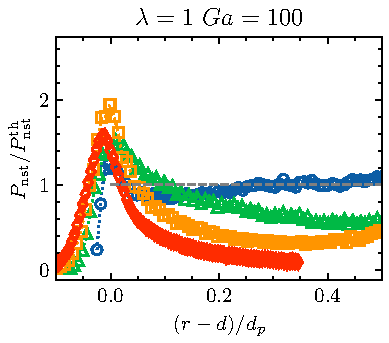
\includegraphics[height=0.3\textwidth]{image/HOMOGENEOUS_NEW/Dist/Pr_l_1_Ga_100.pdf}
    % 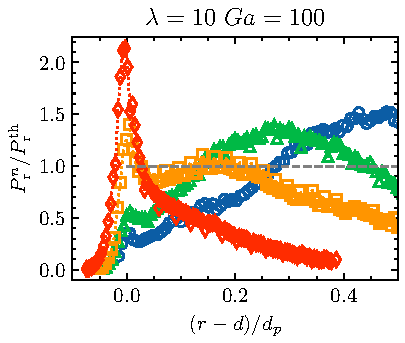
\includegraphics[height=0.3\textwidth]{image/HOMOGENEOUS_NEW/Dist/Pr_l_10_Ga_100.pdf}
%     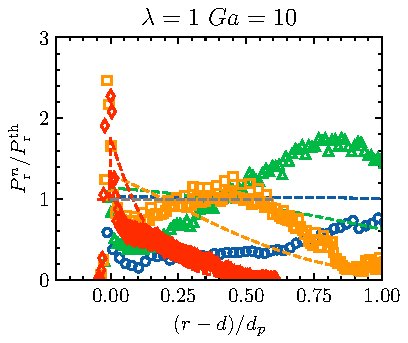
\includegraphics[height=0.3\textwidth]{image/HOMOGENEOUS_NEW/Dist/Pr_l_1_Ga_10.pdf}
%     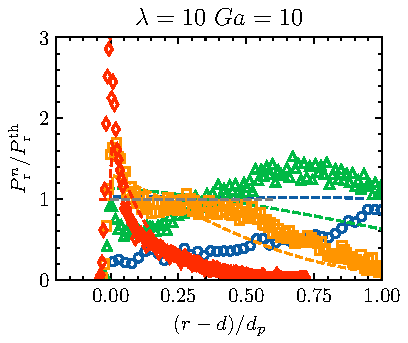
\includegraphics[height=0.3\textwidth]{image/HOMOGENEOUS_NEW/Dist/Pr_l_10_Ga_10.pdf}
%     \caption{Radial probability density function $P_\text{nst}^n(\textbf{x},t,r)$ divided by the theoretical distribution $P_\text{nst}^{th}$ \ref{eq:Pnst_dilute}, in terms of the dimensionless distance $(r-d)/d_p$ where, $d_p = n_p^{-1/3}$, for  $Ga = 10$.
%     (left)  $\lambda = 1$.
%     (right) $\lambda = 10$.
%     ($\pmb\bigcirc$) $\phi = 0.01$; ($\pmb\triangle$) $ \phi = 0.05$; ($\pmb\square$) $\phi = 0.1$ ($\pmb\lozenge$) $\phi = 0.2$.
%     (dashed lines) Theoretical prediction : $P_\text{nst}^n/P_\text{nst}^\text{th} = 1$. 
%     For $r<d$ we arbitrarily set $P_\text{nst}^\text{th} = 1$ so that the distribution can be visualized.
%     }
%     \label{fig:Pr_low}
% \end{figure}
In this appendix we provide additional graph to support the argumentation made in the main text. 
The age distribution for low \textit{Galileo} number is displayed in \ref{fig:age_picture_low_ga}. 
\begin{figure}[h!]
    \centering
    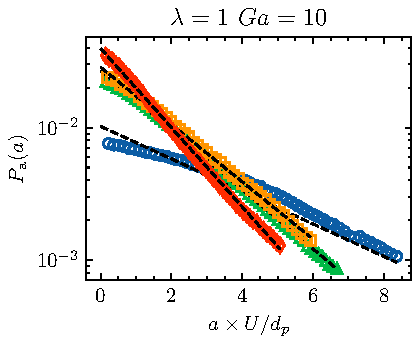
\includegraphics[height = 0.3\textwidth]{image/HOMOGENEOUS_NEW/Dist/Pa_l_1_Ga_10.pdf}
    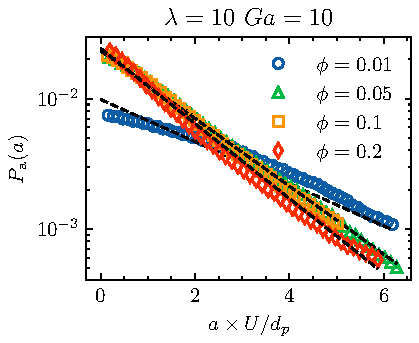
\includegraphics[height = 0.3\textwidth]{image/HOMOGENEOUS_NEW/Dist/Pa_l_10_Ga_10.pdf}
    \caption{(left) Age distribution at $\lambda = 10$ and $Ga = 10$ for : (solid line) $\phi = 0.2$; (dash dotted line) $\phi = 0.1$; (dashed line) $\phi =0.05$; (dotted line) $\phi = 0.01$. 
    (right) Mean dimensionless age in terms of the volume fraction $\phi$ for : 
    ($\pmb\bigcirc$) $Ga=1$; ($\pmb\triangle$) $ Ga = 10$; ($\pmb\square$) $Ga = 50$ ($\pmb\lozenge$) $Ga =100$.
    The age and $\tau_a$ are made dimensionless with $U/d$ where $U$ is the drift-velocity between the dispersed and continuous phase.  }
    \label{fig:age_picture_low_ga}
\end{figure}